% Slide 09 — how the call reaches a phone.
%
% Worth a slide because "a voice agent calls the participant" invites the
% question "calls them how?", and the answer is a real one: the same interface
% drives a browser handset and a real telephone, and the demo picks the first
% because the second costs money per minute.
%
% The fictitious-number guard is the detail to dwell on. It is the difference
% between a demo that could dial a stranger and one that cannot.
\documentclass[border=0pt]{standalone}
% Figure preamble: the shared base plus a transparent page background, so a
% figure composites onto the slide ground instead of carrying a white box.
% Shared preamble for every Reconmed figure and slide.
\usepackage{xcolor}
\usepackage{graphicx}
\usepackage{tikz}
\usetikzlibrary{positioning,calc,fit,backgrounds,shapes.misc,arrows.meta,decorations.pathreplacing}

% Reconmed — presentation palette.
%
% A green medical theme, derived from the product's tokens (frontend/src/styles/
% tokens.css) but with the brand moved to a deep clinical green.
%
% The product's colour rule survives the rebrand unchanged: warm hues (alarm,
% caution) are reserved for prohibited findings and low confidence — never for
% change types. Change types stay cool and are kept off the brand green so the
% brand and the "add" state do not blur together.
\definecolor{ground}{HTML}{EFF4F0}
\definecolor{surf}{HTML}{FFFFFF}
\definecolor{surfii}{HTML}{F6FAF7}
\definecolor{surfiii}{HTML}{E5EDE7}

\definecolor{line}{HTML}{DBE5DD}
\definecolor{lineii}{HTML}{C1D1C4}
\definecolor{lineiii}{HTML}{92A796}

\definecolor{ink}{HTML}{10231A}
\definecolor{inkii}{HTML}{3B4F43}
\definecolor{inkiii}{HTML}{66796D}
\definecolor{inkiv}{HTML}{92A796}

% the brand green
\definecolor{brand}{HTML}{14532D}
\definecolor{brandii}{HTML}{1B6B3A}
\definecolor{brandwash}{HTML}{E8F2EA}

% the participant side of the call — cool and neutral, so the agent's green
% is the only brand colour on the slide
\definecolor{patient}{HTML}{4E6570}

% change types — cool, deliberately unalarming
\definecolor{add}{HTML}{15803D}
\definecolor{stop}{HTML}{6A4C93}
\definecolor{modify}{HTML}{1F5FA8}
\definecolor{same}{HTML}{6B7C70}

% the one loud thing
\definecolor{alarm}{HTML}{C2190B}
\definecolor{alarmink}{HTML}{A3170C}
\definecolor{alarmdim}{HTML}{F1B9B2}
\definecolor{alarmwash}{HTML}{FDF3F1}

% low confidence — dim gold, never red
\definecolor{caution}{HTML}{8A6206}

\definecolor{accept}{HTML}{15803D}
% Rejected is a decision, not an alarm: kept neutral so red stays reserved for
% prohibited findings.
\definecolor{reject}{HTML}{5F6B72}

% Type for the deck.
%
% Two families: Montserrat for headings, big numbers and the wordmark — a
% geometric sans that reads as a health brand — over Open Sans for everything
% else. Keeping the body on Open Sans matters: the dense technical slides were
% measured against it, so the small type does not reflow under the rebrand.
\usepackage{fontspec}
\defaultfontfeatures{Ligatures=TeX}
\setsansfont{Open Sans}
\newfontfamily\displayfont{Montserrat}
\renewcommand{\familydefault}{\sfdefault}

% Shared TikZ styles. Every figure draws in millimetres (x=1mm,y=1mm) on a
% 160x90 canvas, so these sizes are literal.
%
% No blank lines may appear inside the \tikzset below: a blank line is \par,
% and the key parser will not tolerate it.
\tikzset{
  panel/.style     = {draw=line, fill=surf,   line width=0.4pt, rounded corners=2pt},
  panelgray/.style = {draw=line, fill=surfii, line width=0.4pt, rounded corners=2pt},
  screen/.style    = {draw=line, fill=surf,   line width=0.5pt, rounded corners=2.5pt},
  hair/.style      = {draw=line,   line width=0.4pt},
  hairii/.style    = {draw=lineii, line width=0.5pt},
  dimbar/.style    = {fill=line,   rounded corners=0.6pt},
  dimbarsm/.style  = {fill=lineii, rounded corners=0.5pt},
  lab/.style       = {font=\fontsize{7}{8.5}\selectfont\sffamily\color{inkiii}, inner sep=0pt, outer sep=0pt},
  val/.style       = {font=\fontsize{9}{11}\selectfont\sffamily\color{ink},    inner sep=0pt, outer sep=0pt},
  valb/.style      = {font=\fontsize{9}{11}\selectfont\sffamily\bfseries\color{ink}, inner sep=0pt, outer sep=0pt},
  code/.style      = {font=\fontsize{7}{8.5}\selectfont\ttfamily\color{inkiii}, inner sep=0pt, outer sep=0pt},
  tag/.style       = {font=\fontsize{5.6}{6.5}\selectfont\sffamily\bfseries, inner xsep=1.3mm, inner ysep=0.7mm, rounded corners=1.4pt},
  pill/.style      = {font=\fontsize{6.4}{7.5}\selectfont\sffamily\bfseries, inner xsep=1.5mm, inner ysep=0.85mm, rounded corners=1.5pt},
  headline/.style  = {font=\fontsize{12}{14}\selectfont\sffamily\bfseries\color{ink}, anchor=west, inner sep=0pt, outer sep=0pt},
  subline/.style   = {font=\fontsize{7.5}{9}\selectfont\sffamily\color{inkii}, anchor=west, inner sep=0pt, outer sep=0pt},
  cardlab/.style   = {font=\fontsize{6.4}{7.5}\selectfont\sffamily\color{inkiii}, anchor=west, inner sep=0pt, outer sep=0pt},
  num/.style       = {font=\fontsize{22}{23}\selectfont\sffamily\bfseries\color{ink}, anchor=west, inner sep=0pt, outer sep=0pt},
  flow/.style      = {-{Stealth[length=1.5mm,width=1.2mm]}, draw=lineii, line width=0.7pt},
}

% The conmed mark.
%
% Concept: two records — the log on file, and what the participant said —
% converging into a single reconciled line. Drawn once as a standalone asset
% (shared/marks/conmed.tex) so it scales cleanly: PDF inclusion scales the
% strokes, which TikZ scope scaling would not.
\newcommand{\conmedmark}[1][16mm]{
\includegraphics[height=#1]{shared/marks/conmed.pdf}}


\AtBeginDocument{\ifdefined\nopagecolor\nopagecolor\fi}

\begin{document}
\hyphenpenalty=10000\exhyphenpenalty=10000
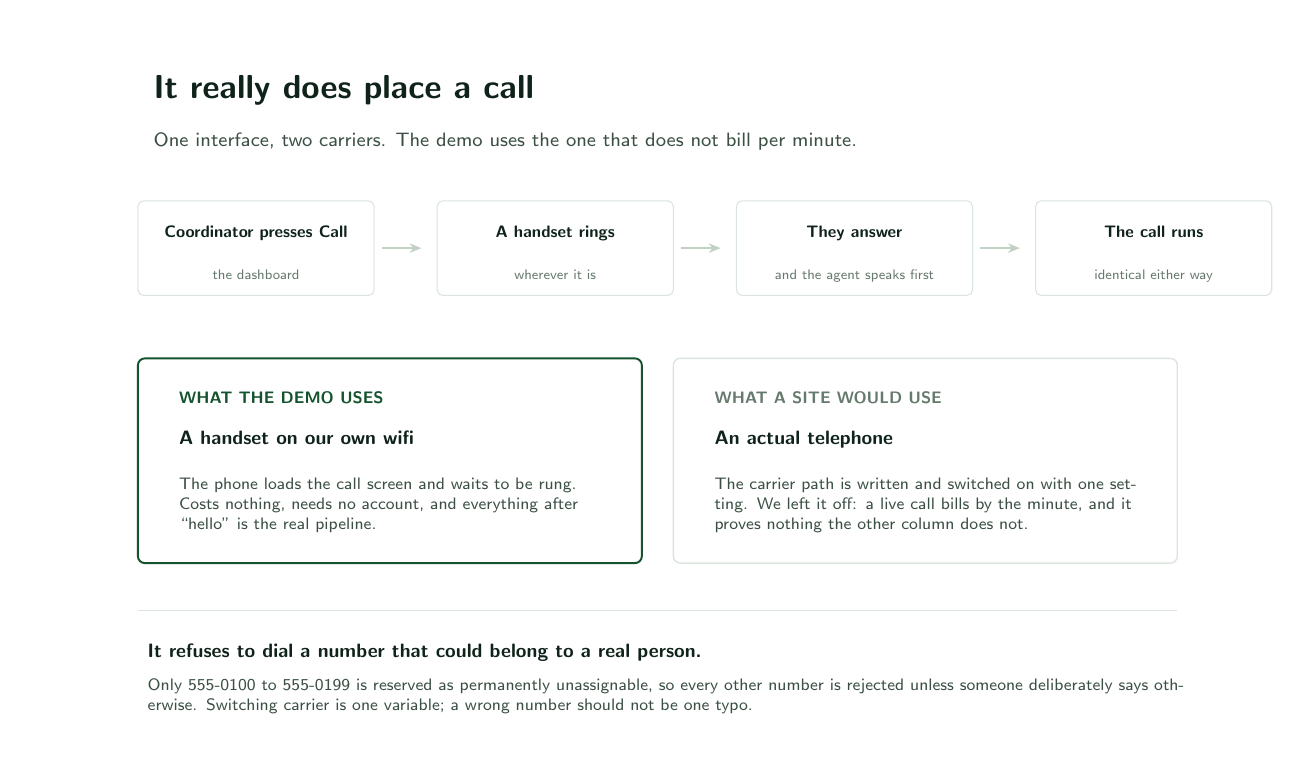
\begin{tikzpicture}[x=1mm,y=1mm]
\path[use as bounding box] (0,0) rectangle (160,90);

\node[headline] at (16,82) {It really does place a call};
\node[subline]  at (16,75.5) {One interface, two carriers. The demo uses the one that does not bill per minute.};

% ---- the flow -----------------------------------------------------------
\foreach \x/\step/\who in {%
  14/{Coordinator presses Call}/{the dashboard},
  52/{A handset rings}/{wherever it is},
  90/{They answer}/{and the agent speaks first},
  128/{The call runs}/{identical either way}}{%
  \fill[surf, rounded corners=2pt] (\x,56) rectangle (\x+30,68);
  \draw[line, line width=0.4pt, rounded corners=2pt] (\x,56) rectangle (\x+30,68);
  \node[anchor=north, font=\fontsize{6}{7.3}\selectfont\sffamily\bfseries\color{ink}, align=center, text width=27mm] at (\x+15,66) {\step};
  \node[anchor=north, font=\fontsize{5.4}{6.5}\selectfont\sffamily\color{inkiii}, align=center, text width=27mm] at (\x+15,60.5) {\who};
}
\foreach \x in {45, 83, 121}{ \draw[flow] (\x,62) -- (\x+5,62); }

% ---- the two carriers ---------------------------------------------------
\fill[surf, rounded corners=2.5pt] (14,22) rectangle (78,48);
\draw[brand, line width=0.7pt, rounded corners=2.5pt] (14,22) rectangle (78,48);
\node[anchor=north west, font=\fontsize{5.6}{6.8}\selectfont\sffamily\bfseries\color{brand}] at (18,45) {WHAT THE DEMO USES};
\node[anchor=north west, font=\fontsize{7.2}{8.8}\selectfont\sffamily\bfseries\color{ink}] at (18,40) {A handset on our own wifi};
\node[anchor=north west, font=\fontsize{5.8}{7.2}\selectfont\sffamily\color{inkii}, align=left, text width=56mm] at (18,34)
  {The phone loads the call screen and waits to be rung. Costs nothing, needs no account, and everything after ``hello'' is the real pipeline.};

\fill[surf, rounded corners=2.5pt] (82,22) rectangle (146,48);
\draw[line, line width=0.5pt, rounded corners=2.5pt] (82,22) rectangle (146,48);
\node[anchor=north west, font=\fontsize{5.6}{6.8}\selectfont\sffamily\bfseries\color{inkiii}] at (86,45) {WHAT A SITE WOULD USE};
\node[anchor=north west, font=\fontsize{7.2}{8.8}\selectfont\sffamily\bfseries\color{ink}] at (86,40) {An actual telephone};
\node[anchor=north west, font=\fontsize{5.8}{7.2}\selectfont\sffamily\color{inkii}, align=left, text width=56mm] at (86,34)
  {The carrier path is written and switched on with one setting. We left it off: a live call bills by the minute, and it proves nothing the other column does not.};

% ---- the guard ----------------------------------------------------------
\draw[line, line width=0.5pt] (14,16) -- (146,16);
\node[anchor=north west, font=\fontsize{6.8}{8.2}\selectfont\sffamily\bfseries\color{ink}] at (14,13)
  {It refuses to dial a number that could belong to a real person.};
\node[anchor=north west, font=\fontsize{5.8}{7}\selectfont\sffamily\color{inkii}, align=left, text width=132mm] at (14,8.5)
  {Only 555-0100 to 555-0199 is reserved as permanently unassignable, so every other number is rejected unless someone deliberately says otherwise. Switching carrier is one variable; a wrong number should not be one typo.};

\end{tikzpicture}
\end{document}
